\documentclass[conference]{IEEEtran}

\usepackage{todonotes}
\usepackage{url}
\usepackage{graphicx}
\usepackage{algorithm}
% \usepackage{algorithmic}
\usepackage{algpseudocode}
\usepackage{amsmath}
\usepackage{amssymb}
\usepackage{amsthm}
\usepackage{colortbl}
% \usepackage[table]{xcolor}

\usepackage{listings}

\usepackage{color}
\definecolor{gray}{rgb}{0.4,0.4,0.4}
\definecolor{darkblue}{rgb}{0.0,0.0,0.6}
\definecolor{cyan}{rgb}{0.0,0.6,0.6}

\lstset{
  basicstyle=\ttfamily\small,
  columns=fullflexible,
  showstringspaces=false,
  commentstyle=\color{gray}\upshape
}

\lstdefinelanguage{XML}
{
  morestring=[b]",
  morestring=[s]{>}{<},
  morecomment=[s]{<?}{?>},
  stringstyle=\color{black},
  identifierstyle=\color{darkblue},
  keywordstyle=\color{cyan},
  morekeywords={xmlns,version,type}% list your attributes here
}

\newcounter{eqn}
\renewcommand*{\theeqn}{\alph{eqn})}
\newcommand{\num}{\refstepcounter{eqn}\text{\theeqn}\;}

\makeatletter
\newcommand{\putindeepbox}[2][0.7\baselineskip]{{%
    \setbox0=\hbox{#2}%
    \setbox0=\vbox{\noindent\hsize=\wd0\unhbox0}
    \@tempdima=\dp0
    \advance\@tempdima by \ht0
    \advance\@tempdima by -#1\relax
    \dp0=\@tempdima
    \ht0=#1\relax
    \box0
}}
\makeatother

\begin{document}

\title{Bitcoin Boomerang \\ {\LARGE Collaborative Anonymity for Transaction Broadcasting}}

\author{\IEEEauthorblockN{Christopher A. Wood}
\IEEEauthorblockA{Department of Computer Science\\
University of California Irvine\\
Email: woodc1@uci.edu}
\and
\IEEEauthorblockN{Chris H. Vu}
\IEEEauthorblockA{Department of Computer Science\\
University of California Irvine\\
Email: ChrisHVu@gmail.com}}

% make the title area
\maketitle

\begin{abstract}
Sender anonymity is important in the design of several ``cryptographically-enhanced'' variations of Bitcoin, such as ZeroCoin \cite{zerocoin}. Consequently, they often state that users install and use network-layer anonymity layers such as Tor \cite{tor} alongside their existing Bitcoin clients when introducing new transactions into the network. Such requirements make such variations less appealing from a usability perspective. Furthermore, since low-latency anonymity layers like Tor are susceptible to strategic timing attacks by adaptive global adversaries, and transactions do not have real-time constraints in which they must be broadcasted throughout the network, mixnets are a more appropriate solution for achieving sender anonymity. To this end, we introduce Bitcoin Boomerang, a distribtued, collaborative, application-level protocol for achieving mixnet-like behavior to increase sender anonymity. Boomerang is intended to run at the application-layer \emph{within} Bitcoin software clients as an extension of the Bitcoin protocol. We analyze the anonymity properties of Boomerang, and assess the induced performance overhead using a custom simulator that emulates the behavior of Bitcoin nodes (software clients) adhering to the protocol. Our preliminary results indicate that with appropriate parameter tuning, increased sender anonymity with a single software client can be achieved for the small price of increased computational overhead and network bandwidth consumption for each participating Bitcoin user.
\end{abstract}

\IEEEpeerreviewmaketitle

\section{Introduction}
%TODO: general overview of cryptocurrency, bitcoin (why it's unique), and a summary of problems it suffers from

Electronic commerce would benefit greatly from the existence of a completely secure, private, and anonymous form of digital currency that does not rely on trusted third parties or external financial institutions to manage transactions. Motivated by this ideal type of currency, there have been many research efforts focused on generating suitable cryptography-based digital payment systems, or cryptocurrencies, such as DigiCash \cite{digicash}, E-Cash \cite{ecash}, HashCash \cite{hashcash}, Namecoin \cite{namecoin}, Peercoin \cite{peercoin}, Litecoin \cite{litecoin}, Ripple \cite{ripple}, and perhaps the most popular variant, Bitcoin \cite{bitcoin}. Each of these schemes offer different tradeoffs of security, privacy, and anonymity, and as such have varying popularity among users. However, it is the distribtued, decentralized nature of Bitcoin that has led to its widespread popularity among the general public and research communities \cite{news articles}. 

Bitcoin is distinguished from other cryptocurrencies by the fact that it does not rely on trusted third parties. Specifically, the global and publicly accessible ledger that stores records of all financial transactions, thereby serving as a verifiable history of all Bitcoin funds in circulation, is maintained by a widely distributed, peer-to-peer network of (untrusted) users. Transactions are linked to specific identities, or pseudonyms, via digital signatures used to ensure the validity of each transaction. In this context, it is often convenient to associate specific pseudonomous addresses with a single public and private key pair owned by a particular user. Unfortunately, these pseudonoyms are very weak masks for the underlying user's identity - user privacy and anonymity are still at risk even with the use of such pseudonomous identities. This is true even if a user has multiple pseudononyms and uses them with caution to deter attackers looking for such links. Consequently, user deanonymization is a major problem for Bitcoin users, and there have been several academic efforts to further the cause for Bitcoin user privacy and anonymity, including studies by Reid and Harrigan \cite{ReidHarrigan13} and Androulaki et al. \cite{Androulaki12-privacy}, and we can expect to see similar work publishing in the coming years. Elias \cite{8} also discussed some legal, and moral, aspects of the anonymity, or lack thereof, in Bitcoin. We do not focus on such legality issues here, and merely operate under the assumption that spender anonymity is an ideal property that any currency system should have.

Currently, techniques to address such anonymity issues with Bitcoin are rather limited and include the use of Chaumian's entirely independent e-cash system \cite{chaumain}, which relies on trusted third parties, and Zerocoin \cite{zerocoin}, which achieves privacy and anonymity properties based on strong cryptographic assumptions at the protocol-level by working \emph{on top of} Bitcoin, among others. The former is not ideal for several reasons; the most significant of which is that it directly conflicts with the decentralized nature of Bitcoin. The latter technique is very young, having only been published in the past year, and is just now starting to gain considerable attention \cite{pinocchio}. 

In this work we survey Bitcoin and related forms of cryptocurrency with respect to their privacy and anonymity properties. We analyze proposed solutions and offer critical insight into the open problems and difficulties in achieving perfect privacy and anonymity with minimal resource consumption (e.g., bandwidth, CPU cycles, etc.). We hope that this survey will motivate continued research on this critical problem that has the potential to change financial instutitions and forms of currency for future generations.

\todo[inline]{outline the sections here}
\section{Bitcoin Overview and Privacy Limitations}
% TODO: specific discussion of aspects of bitcoin that pertain to privacy/anonymity

TODO: intro

\subsection{Bitcoin Basics}

Bitcoin is a distributed, decentralized form of cryptocurrency. Accordingly, this enables all (digitally signed)  transactions between two parties to be conducted in a peer-to-peer fashion without the inclusion of a trusted third party, such as a bank or other financial institution. This form of decentralized exchange comes at a price, however, as there must be some way to prevent users from \emph{double spending}, or using the same funds to simultaneously pay multiple parties. Bitcoin achieves this property by relying on its users to construct a history for every transaction that takes place in the system. If a majority of the users accept the validity of a particular transaction, or a set of transactions, the global history of the system is affirmatively updated and ``confirmed'' via a cryptographic hash digest that all users agree upon. This hash digest, referred to as a hash-based proof-of-work, is what constitutes the validity of the system. By the properties of the underlying hash function, the history of the system cannot be changed without breaking the function (i.e., finding collisions) or re-doing the proof-of-work, which is computationally infeasible for small groups of nodes. Therefore, so long as a majority of the Bitcoin users are honest, the system history is deemed correct and thus all signed transactions are verified, preventing double spending by potentially malicious users participating in direct, peer-to-peer transactions. 

Unfortunately, while the above scheme is semantically correct and provides strong guarantees that all financial transactions are valid, there are inherent limitations in the amount of user privacy and anonymity that can be achieved in Bitcoin. In order to adequately define these limitations, we first describe how Bitcoin transactions are generated and how the system history is maintained. For simplicity, consider the scenario in which user $A$ wants to send $N$ BTCs (Bitcoins) to user $B$. Rather than identify users by name, Bitcoin uses \emph{addresses} that are tied to specific users to use in such transactions. Denote $\mathsf{addr}_A$ and $\mathsf{addr}_B$ as the addresses of users $A$ and user $B$ used in this transaction. It is often convenient to think of Bitcoin addresses as public keys $\mathsf{pk}_A$ and $\mathsf{sf}_B$, and as such there are corresponding private keys, which we denote as $\mathsf{sk}_A$, and $\mathsf{sk}_B$, respectively.

Structurally, a transaction $T$ is a tuple comprised of the \emph{source} transactions which supplied the funds necessary to make this transaction, denoted as $\mathsf{source}$, the (public) address of the recipient, $\mathsf{addr}_B$, the amount of BTCs to send, $N$, and a digital signature of these three properties, $\mathsf{Sign}_{\mathsf{sk_A}}({\mathsf{source}, \mathsf{pk}_B, N})$. In other words, we have 
\begin{align*}
T = (\mathsf{source}, \mathsf{pk}_B, N, \sigma), 
\end{align*}
where $\sigma = \mathsf{Sign}_{\mathsf{sk_A}}({\mathsf{source}, \mathsf{pk}_B, N})$. Note that this signature is embedded in $T$ so that any other Bitcoin user may verify the validity of the content using $\mathsf{pk}_A$. Also note that $\mathsf{source}$ need not be a single transaction; user $A$ is free to use multiple transactions in order to fund their transaction to $B$. In addition to the $N$ BTC transfer from $A$ to $B$, there is often $C$ BTC amount specified in the transaction for a particular address, where $C$ denotes the amount of change that will be given to this address as a result of the transaction. It is not required that the address to which $C$ is addressed is the same as the address of $A$, though this often happens in practice. Figure \ref{fig:transaction-io} illustrates the input and output relation of our transaction from $A$ to $B$, and Figure \ref{fig:transaction-create} illustrates the steps used in constructing this transaction. Note that, in both cases, $\mathsf{source}$ is comprised of two transactions $T_1$ and $T_2$, and the resulting transaction is denoted as $T_3$.

\begin{center}
\begin{figure}
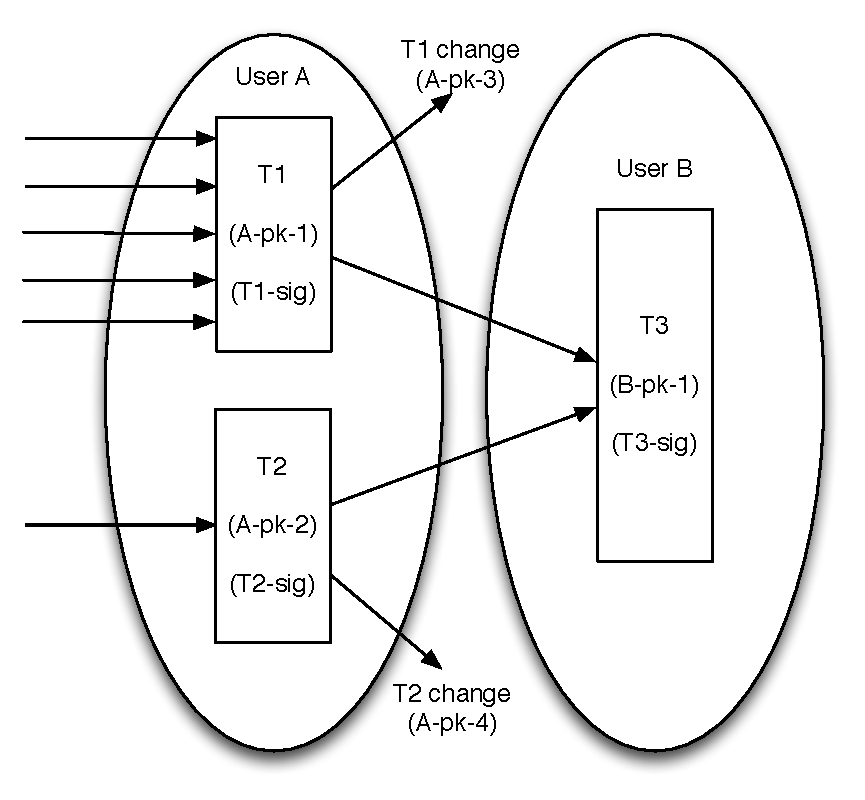
\includegraphics[scale=0.5]{./images/transaction_io.pdf}
\caption{Visual depiction of the input and output elements of a transaction from user $A$ to user $B$.}
\label{fig:transaction-io}
\end{figure}
\end{center}

\begin{center}
\begin{figure}
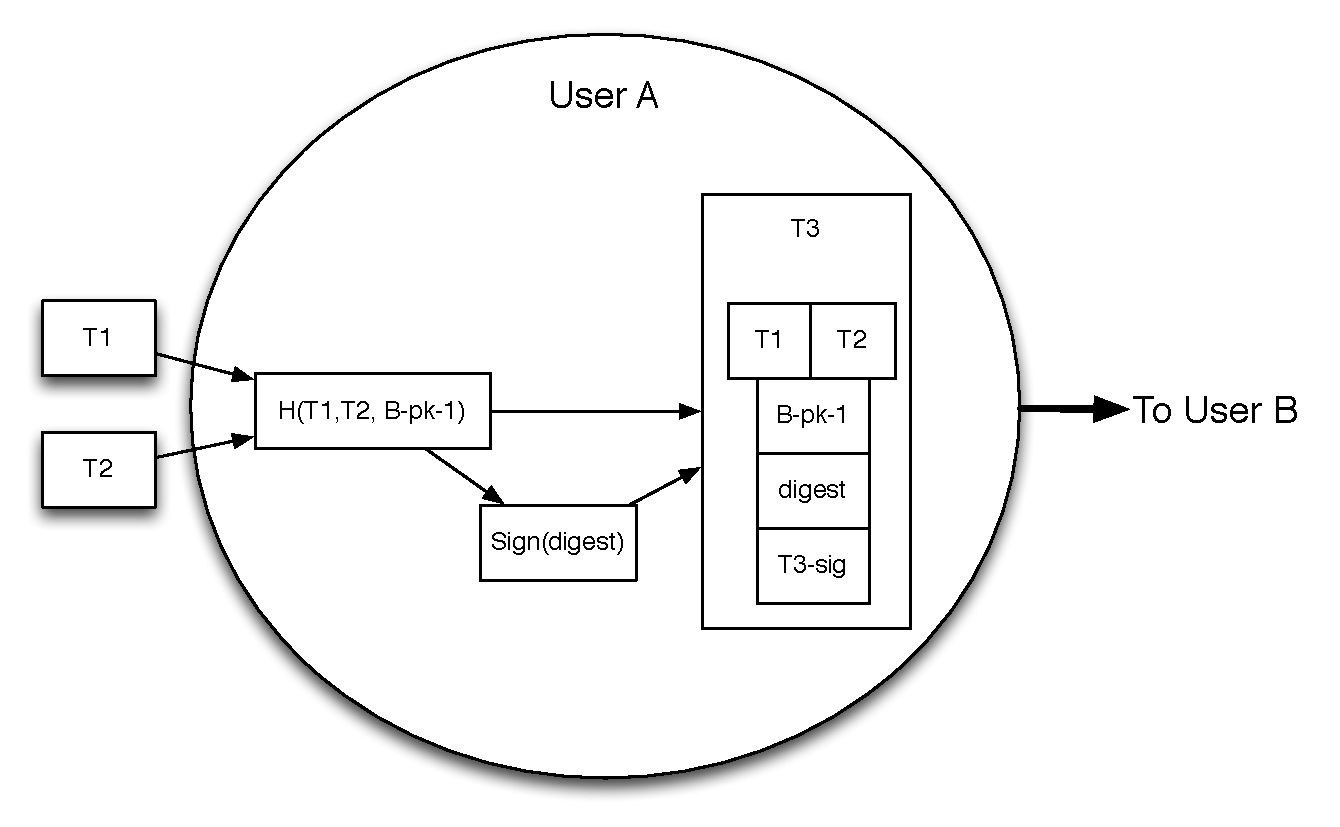
\includegraphics[scale=0.4]{./images/transaction_create.pdf}
\caption{Visual depction of the steps to create a transaction $T_3$ from user $A$ to user $B$ using two input transactions, $T_1$ and $T_2$.}
\end{figure}
\end{center}

After a transaction has been created, it is broadcasted in the network. In order to prevent double spending, nodes must confirm this transaction and append it to the chain of accepted transactions in the system's history. This procedure is based on the aforementioned proof-of-work, which works as follows. Bitcoin miners will collect unconfirmed transactions into a buffer, along with the longest chain of system-wide accepted transactions, and compute a Merkle hash of the transactions and digest of the chain. The output digest of this Merkle hash, referred to as the challenge $c$ in the proof-of-work protocol, is then used to find the proof $p$. Together, $c$ and $p$ have the property that, when concatenated and hashed using a cryptographically strong collision-resistant hash function $H$, the leading $B$ bits of the output $x = H(c || p)$ are all $0$. That is, $x = \{0,1\}^B\{0,1\}^{256-B}$. Given the collision resistant properties of $H$, finding a valid proof $p$ for the challenge $c$ is comptuationally difficult. Figure \ref{fig:block} illustrates the construction of $c$ and $p$ using a previously confirmed block chain $B$.

Once a miner finds a proof, it is broadcasted to the other nodes in the network along with the input transactions used by the miner, who can then easily recompute the challenge $c$ and verify the correctness of $p$. Once verified, this new transaction ``block'' is appended to the block chain which the miner used in finding the proof. Miners will continually use the longest block chain to gather and verify transaction blocks. Since there is a particular subset of BTCs in each transaction that are paid to the miner who provides the proof-of-work for a block containing that transaction, referred to as the transaction fee, miners are financially incentivized to collect more transactions into a block and continually ``mine'' for valid proofs-of-work. 

\subsection{Privacy Limitations}
TODO



\section{Boomerang Design}

As previously discussed, the Boomerang protocol enhancement for Bitcoin is motivated by the need to hide the source from which transactions are introduced into the network. Furthermore, this should be done in a transparent way so that any other form of anonymous coin extension on top of Bitcoin (e.g., Zerocoin) can leverage the service for transaction anonymity. Boomerang is \emph{not} intended to support regular Bitcoin traffic; once a transaction becomes public knowledge, Boomerang no longer plays a role in its distribution. 

In the following sections we detail the core protocol and several important design and security tradeoffs that can be made in practice when using Boomerang. A formal analysis of the security and performance of Boomerang-enhanced Bitcoin is provided in Sections X and Y. 

\subsection{Broadcast Protocol}

At the heart of the Bitcoin protocol is the ability to encode new transactions as Boomerang messages and then ripple them throughout the network. We describe the complete procedure for message encoding, {\sf EncodeTransaction}, in Algorithm \ref{alg:encode}, where the notation contained therein is defined in Table \ref{tab:notation}. An encoded Boomerang message has a very well-defined format, as shown in Figure \ref{fig:boomerang_message}. In particular, the message is composed of the following:
\begin{enumerate}
	\item A potentially re-encrypted seed. By the description of {\sf EncodeTransaction}, it is required that the public-key encryption scheme used to mask these seeds has the same domain and range. This is needed because the decrypted seed for one hop will be used as decrypted seed on the previous hop, very much like onion layers of encryption.
	\item An encrypted address vector that is used by each hop to learn the next hop in the circuit without learning any other information about the nodes in the circuit. More specifically, a router can only learn about the immediate source and destination of a Boomerang message (the security and anonymity implications of this are discussed in the following section).
	\item A potentially re-encrypted transaction message block. This block either stores the encrypted transcaction, where the encryption is done by XORing with a pseudorandom bit string generated by the decrypted seed value, or the plaintext transaction that is to be broadcast throughout the network.
\end{enumerate}

\begin{figure}[ht!]
\begin{center}
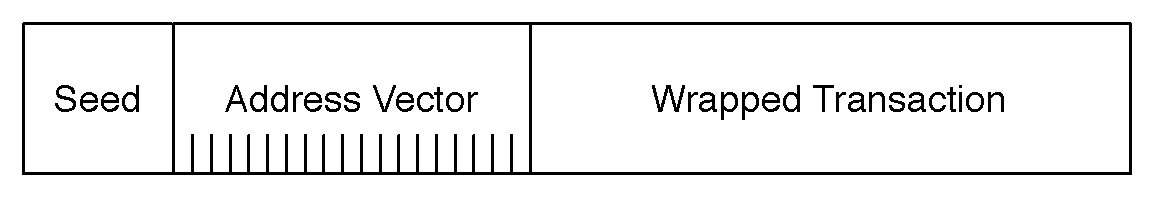
\includegraphics[scale=0.4]{./images/boomerang_message.pdf}
\caption{Boomerang message encoding.}
\label{fig:boomerang_message}
\end{center}
\end{figure}

The procedure to handle Boomerang messages, {\sf BoomerangMessageHandler}, is provided in Algorithm \ref{alg:handler}. 

\begin{algorithm*}[t!]
\caption{{\sf EncodeTransaction}($T$)}
\label{alg:encode}
\begin{algorithmic}[1]

\For{$m = 1$ to $M$}
	\State $\bar{T} := T$
	\State $s \gets \{0,1\}^{\tau}$
	\For{$n = 1$ \textbf{to} $N_m$}
		\State $p := \mathsf{PRG}(s)$
		\State $\bar{T} := \bar{T} \oplus p$
		\State $s \gets E_{pk_{m,n}}(s)$
	\EndFor

	% populate the address vector
	\State $\mathsf{index} \gets \{0,\dots,2N_m\}$ % random address vector index
	\State $\mathsf{AV} := [2N_m]$ % address vector
	\For{$n = N_m$ \textbf{downto} $2$}
		\State $\mathsf{AV}[\mathsf{index}] := E_{pk_{m,n}}(\mathsf{addr}_{N_n})$
		\State $\mathsf{index} := \mathsf{index} + 1 (\mod N_m)$
		\State $\mathsf{AV}[\mathsf{index}] := E_{pk_{m,n}}(\mathsf{addr}_{N_{n-1}})$
		\State $\mathsf{index} := \gets \{0,\dots,2N_m\}$
		\While {$\mathsf{index} \mod 2 \not= 0$ \text{ and } $\mathsf{AV}[\mathsf{index}] \not= \bot \text{ and } \mathsf{AV}[\mathsf{index + 1 (\mod N_m)}] \not= \bot$}
			\State $\mathsf{index} \gets \{0,\dots,2N_m\}$
		\EndWhile
	\EndFor

	\State $M := \mathsf{Pack}(s, \mathsf{AV}, \bar{T})$
	\State $\mathsf{Transmit}(M)$
\EndFor

\end{algorithmic}
\end{algorithm*}

\begin{algorithm*}[t!]
\caption{{\sf BoomerangMessageHandler}($n$, $M$)}
\label{alg:handler}
\begin{algorithmic}[1]

\State $s := D_{sk_{n}}(M[0])$
\State $\bar{T} := M[2] \oplus PRG(s)$
\If {$\bar{T}$ is a well formed transaction}
	\State $\mathsf{Broadcast}(\bar{T})$ to the Bitcoin network
\ElsIf {$\bar{T}$ destination address is $\mathsf{addr}_n$}
	\State Discard $\bar{T}$; return;
\Else
	\State $\mathsf{AV} := M[1]$
	\State $n := 1$
	\While {$n < 2N_m$}
		\State $\mathsf{addr}_{src} := D_{pk_n}(AV[n])$
		\If {$\mathsf{addr}_{src} = \mathsf{addr}_n$}
			\State $\mathsf{addr}_{dst} := D_{pk_n}(AV[n + 1])$
			\State $M := \mathsf{Pack}(s, \mathsf{AV}, \bar{T})$
			\If {$|Buffer| \geq B$}
				\State $\mathsf{Transmit}(M)$
			\Else
				\State $B.add(M)$
			\EndIf
		\Else
			\State $n := n + 2$
		\EndIf
	\EndWhile
\EndIf

\end{algorithmic}
\end{algorithm*}

TODO: cover traffic generation, mix delay

\subsection{Cryptographic Primitives}

TODO: PRG, PK-encryption, etc

% \begin{figure}[ht!]
% \begin{center}
% 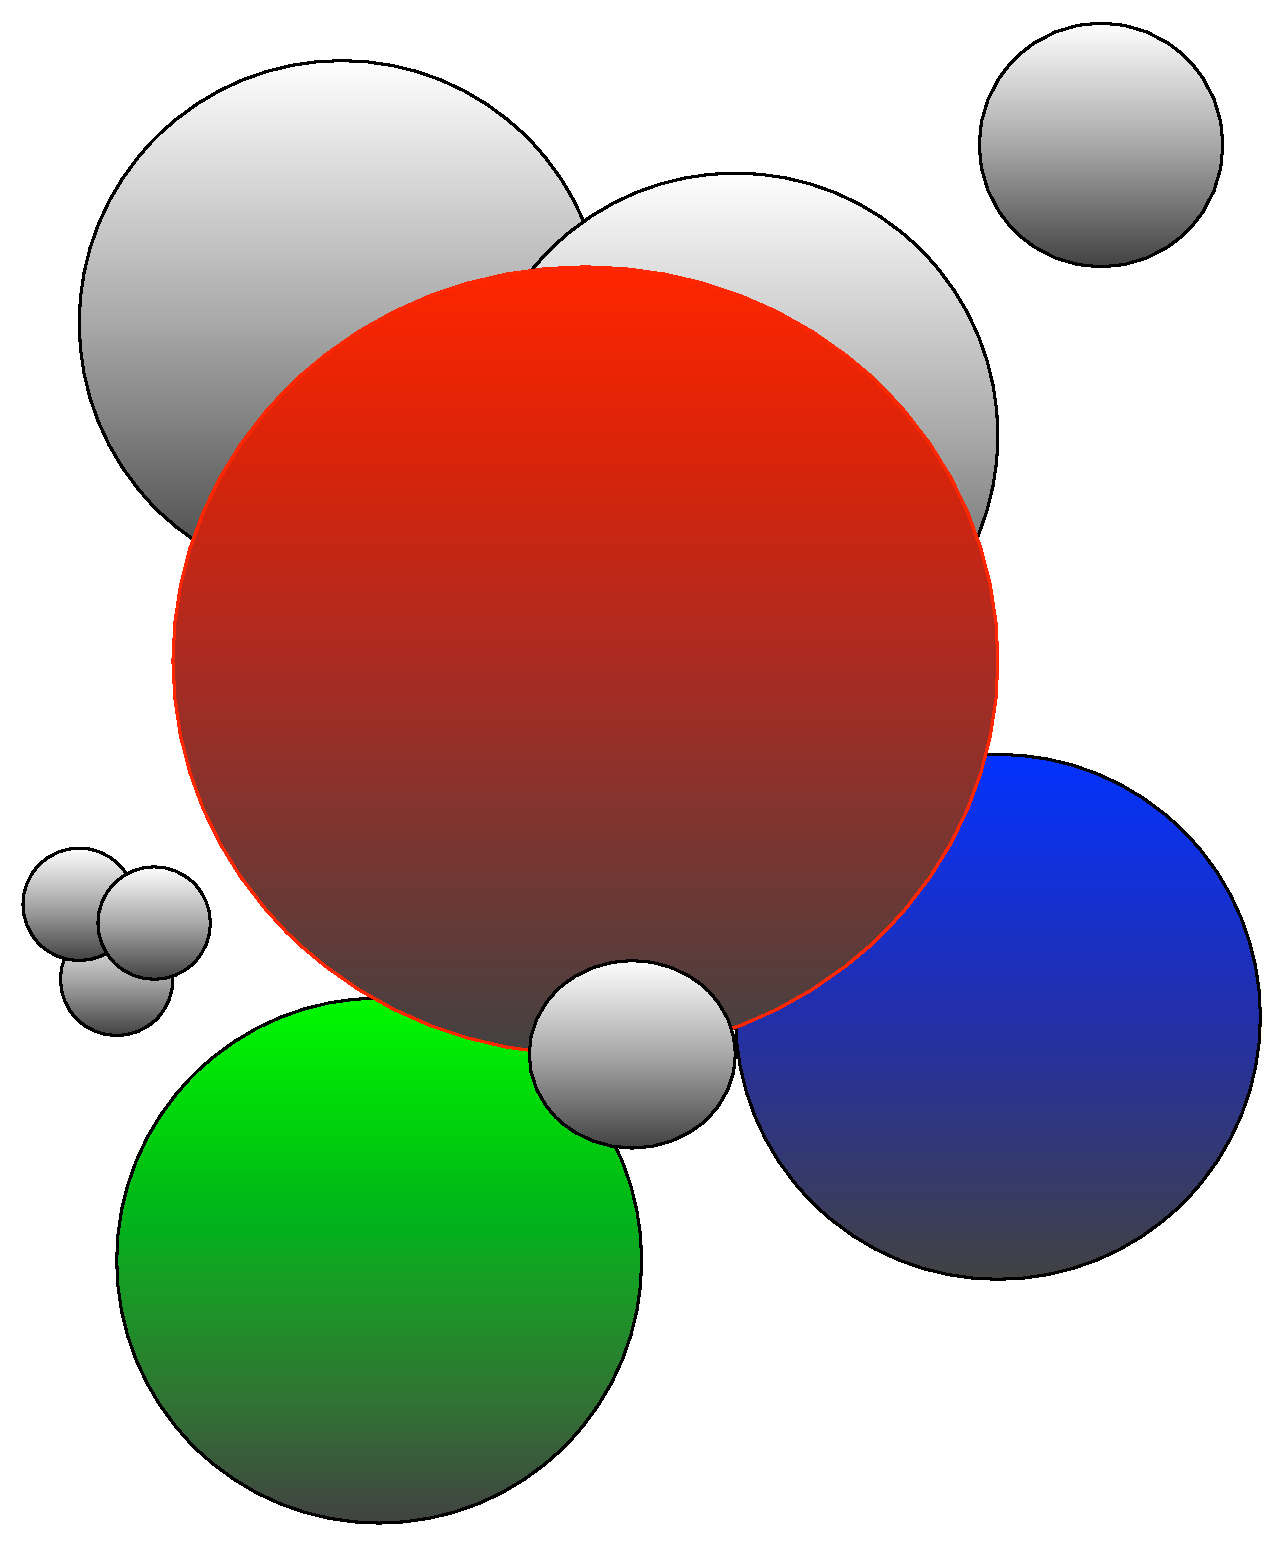
\includegraphics[scale=0.25]{./images/boomerang_clusters.pdf}
% \caption{TODO}
% \label{fig:boomerang_clusters}
% \end{center}
% \end{figure}

\subsection{Parameter Selection}

TODO: discuss parameter selection from below

% cover traffic generation rate (random variable)
% mix buffer delay (random variable)
% circuit length (fixed)
% mix buffer size (fixed)
% encoded transaction size


\section{Boomerang Properties} \label{sec:properties}
In this section we elaborate on the design goals of Boomerang. We first discuss the anonymity properties that are provided by Boomerang, and then discuss system-level properties such as fault tolerance and performance.

\subsection{Anonymity Properties}
Inspired by Tarzan \cite{tarzan}, we analyze the anonymity properties of Boomerang with respect to static and adaptive adversaries. In particular, we strive to show that senders achieve anonymity against a minority of colluding nodes. Before proving any claims, we present the main sources of information exposure in Table \ref{tab:anonymity-properties}; a positive entry indicates that an attacker will be able to uncover the source of information, whereas a negative entry indicates that such exposure is not feasible given the Boomerang design.

\begin{table*}[t]
\begin{center}
	\caption {Boomerang information exposure.}
    \label{tab:anonymity-properties}
    \begin{tabular}{|l||c|c|c|c|}
    \hline
    \emph{Information Exposed} & \emph{Bad Entrance Node} & \emph{Bad Intermediate Node} & \emph{Bad Exit Node} & \emph{Bad Entrance/Exit Nodes} \\ \hline \hline
    Sender activity & Maybe    & Maybe & No & Maybe \\ \hline
    Sender content  & No       & No    & No & Maybe \\ \hline
    \end{tabular}
\end{center}
\end{table*}

% 2. Anonymity against malicious nodes: Tarzan should pro- vide sender or recipient anonymity against colluding nodes. That is, a particular host should not be uniquely linkable as the sender (recipient) of any message, or that a message should not be linkable to any sender (recipient) [20]. We consider these properties in terms of an anonymity set: the set of possible senders of a message. The larger this set, the “more” anonymous an initiator remains. These properties implies the weaker relationship anonymity: an adversary should not be able to identify a pair of hosts as communicating with each other, irrespective of which host is running Tarzan.

One of the defining properties of Boomerang messages is that both encoded transactions and dummy messages are computationally indistinguishable. Therefore, an eavesdropping adversary cannot deterministically determine the type of messages based soley on passive observation, thus ensuring that the contents of each packet are not leaked in the network. Furthermore, even if an adversary successfully differentiates cover traffic from encoded (wrapped) transactions, an adversary cannot determine whether or not a compromised node is forwarding a transaction or is the original source of the transaction.

More formally, the size of the sender anonymity set for any particular message is exponential in the path length, i.e., in a network of $N$ nodes comprised of $N_{bad}$ nodes, there are $((N - N_{bad}) / N)^{i-1}$ possible sending nodes (the size of the anonymity set) of a message at hop $i$ that could have generated the original message, assuming uniformly random and unbiased circuit creation. As a result, the probability that a node $n$ is the originator for a particular message $m$ if intercepted at hop $i$ in the circuit is $((N - N_{bad}) / N)^{-(i-1)}$. Building upon the anonymity analysis completed for Tarzan, we may quantify the confidence that a specific node in the anonymity set is the real sender is precisely as follows:
\begin{align*}
C_i = \frac{\Pr[I_i | H_{i+}]}{E(|AS_i|)},
\end{align*} 
where $|AS_i| = ((N - N_{bad}) / N)^{i-1}$ and $\Pr[I_i | H_{i+}]$ is the probability that \emph{some} node preceding the node at hop $i$ is the sender. In this context, we use $I_i$ to denote the event that a node preceding node $i$ is the original sender, $H_i$ to denote the event that first compromised node occurs at the $i$-th hop, and $H_{i+}$ to be the event that the first compromised node occurs somewhere after the $i$-th hop. Mathematically, we may model the former probability as follows:
\begin{align*}
\Pr[I_i | H_{i+}] & = \frac{\Pr[H_i]}{\Pr[H_{i+}]},
\end{align*}
where
\begin{align*}
\Pr[H_i] = \left( \frac{ \Pr[l \geq i - 1 + E(r)] } { \Pr[l \geq E(r)] }\right) \left(\frac{N - N_{bad}}{N}\right)^{i-1} \left( \frac{N_{bad}}{N}\right)
\end{align*}
and 
\begin{align*}
\Pr[H_{i+}] = \sum_{k=i-1}^{D} \left( \frac{ \Pr[l \geq k + E(r)] } { \Pr[l \geq E(r)] }\right) \left(\frac{N - N_{bad}}{N}\right)^{k} \left( \frac{N_{bad}}{N}\right),
\end{align*}
where $E(r)$ is the expected minimum length of the circuit and $l$ is the length of the circuit.

Analyzing this confidence in the limit as $N_{bad}/N \to 1$, we can see $C_1 \to 1$ (see Figure \ref{fig:confidence-plot}). However, by the assumptions of the Bitcoin network, the number of honest nodes will always be a majority of the total nodes in the network. Making this substitution, we see that the expected size of the anonymity set is $E(|AS_i|) \leq \left(\frac{1}{2}\right)^{i-1}$, in the worst case. $C_i$ also reduces to the following:
\begin{align*}
C_i & = \frac{\Pr[I_i | H_{i+}]}{E(|AS_i|)} \\
& = \frac{\left( \frac{ \Pr[l \geq i - 1 + E(r)] } { \Pr[l \geq E(r)] }\right)}{\sum_{k=i-1}^{D} \left( \frac{ \Pr[l \geq k + E(r)] } { \Pr[l \geq E(r)] }\right) \left(\frac{N - N_{bad}}{N}\right)^{k}}
\end{align*}

%%% TODO: plot the above equation
%%% TODO: change Pr(frac) to \Pr[path travels through i-1 honest nodes] and \Pr[path doesn't travel through k >= i nodes]
%%% TODO: get rid of event I_i, just use H_i's (newly defined as above)

% leakage in tunnels:
% Cover traffic (dummy traffic) that is indistinguishable from data can prevent such analysis. First, an eavesdropper cannot determine whether a relay initiates new data or just sends cover packets. Sec- ond, an observer must back-trace the multiple sources of a node’s incoming traffic, creating a fan-out of possible senders.

% exit/entrance nodes:
% While cover traffic and layered encryption protects data traffic within tunnels, an adversary may attempt to leverage the fact that data exits the Tarzan network in clear-text. These network-edge attacks include packet replay, tagging, reordering, and flooding. They generally require an adversary to control some node or link on a tunnel and to observe a PNAT or the non-participating Internet host of interest. 
% While Tarzan is less susceptible to such attacks on its sender anonymity due to its lack of any entrance points,
% Lastly, an adversary may attempt to flood a node with packets. It hopes to reduce the number of other senders that can simultane- ously use the relay, and then try to identify its own outgoing pack- ets from those of others. Tarzan greatly reduces the effectiveness of such flooding. First, mimics encrypt messages between them, mak- ing it difficult for an adversary to identify its own packets. Second, cover traffic cannot be distinguished from the legitimate traffic of other nodes. Third, the rigid structure of the mimic overlay limits the set of nodes that an adversary attack: A malicious node can only flood mimics through a well-formed tunnel in the overlay.

\subsection{System-Level Properties}
From a systems perspective, Boomerang was designed with fault-tolerance and performance in mind. In particular, we (easily) claim that the Boomerang scheme is resistant to any adversarial attempt to leverage a successful denial of service (DoS) attack on the network. By the assumptions of the Bitcoin network, a majority of the participating nodes will always be honest (i.e., effectively uncompromised). Now, assume that there are $N_{total}$ total nodes in the Bitcoin network, at least $N_{total}/2$ such nodes are honest, and $N_{bad} \leq T/2 - 1$ nodes are compromised. By this claim, during node selection and circuit formation, $W$ nodes will be drawn at random without replacement, meaning that the probability of forming a circuit with at least one corrupt node, in the worst case, is

\begin{align*}
\sum_{i=1}^D \frac{N_{bad}}{(N_{total}/2) - 1 - i}
\end{align*}

For reasonable measures of fault-tolerance, we require that this probability is kept as small as possible. However, for anonymity purposes, we require that $D$ is maximized to achieve optimal mixing (and thus, anonymity) throughout the network. 

\todo[inline]{need to quantify anonymity in terms of $N$ and $T$.}

From a performance perspective, our main goal is to minimize the overhead of Boomerang message encoding, transmission, and forwarding while maximizing the anonymity properties discussed in the previous section. To that end, we discuss how the performance varies based on system-wide parameters that influence such anonymity properties. Based on the Boomerang design it is clear that the performance of the Boomerang scheme is tightly coupled to the following paramters:
\begin{itemize}
	\item $W$ - the circuit width,
	\item $D$ - the circuit depth,
	\item $\sigma$ - the average cover traffic generation rate, and
	\item $\pi$ - the average rate at which new transactions are made.
\end{itemize}

\todo[inline]{How many messages should a node expect to receive in a set amount of time?}


\subsection{Network Security Analysis}
Analysis assumes a client’s first connection is to an honest node. If the client first connects to a malicious node, no security is possible as the malicious node will trivially keep the client in the malicious network. The adversary can use many long-lived identities to bias the distribution of nodes towards the malicious network. If the adversary controls a majority of nodes, no security guarantees are possible.  Therefore, security analysis will assume a client node to be connected to some honest nodes and the adversary does not control the majority of nodes.

The adversary can introduce many invalid addresses into the network. By using Boomerang messages to validate addresses, honest nodes can aggressively prune invalid addresses from their internal databases. In a similar fashion, Boomerang messages will prune nodes that improperly modify data that is routed through them. Due to the open nature of the Boomerang network, no solution to denial-of-service attacks are currently possible.

% 4. Performance: Tarzan should maximize the performance of tunnel transmission, subject to our anonymity requirements, to make Tarzan a viable IP-level communication channel.


\section{Simulations and Performance Analysis}
In this section we describe the implementation of our simulator and discuss some performance measurements acquired using this tool. We also describe features that should be added to the simulator to support more realistic experiments. We conclude with a discussion of good parameter selection based on our observations using the simulator.

\subsection{Simulation Design}
To assess the expected overhead introduced by Boomerang we implemented a custom discrete-time simulator that emulates the behavior of Bitcoin nodes (software clients) running Boomerang. Time in the simulation is measured in epochs; at every epoch a series of events occurs that advances the state of the system in some (usually) deterministic way. Our simulator supports the following behavior to closely resemble Boomerang:
\begin{enumerate}
	\item Nodes enter and exit the network at random times. 
	\item Nodes make new transactions using configuration-specificed parameters $W$ and $D$ at a random rate $\pi$.
	\item Nodes generate cover traffic at a random rate $\sigma$.
	\item Nodes manage their internal address address books according the protocol described in section \ref{sec:design}.
\end{enumerate}

In addition, the simulation dynamically computes the following performance metrics:
\begin{enumerate}
	\item Average number of ``computations'' done per node (i.e., the number of public-key encryption operations to encode a transaction).
	\item Total and average message latency from the start to end of a circuit for single and every message, respectively.
	\item Node forwarding throughput (messages/s).
	\item Number of completed messages (transactions and cover messages) vs the number of in-progress messages.
	\item Average number of transaction broadcast retries per node.
\end{enumerate}

The parameters for a particular simulation are specified via a YAML configuration file which is parsed using the Java-based JYaml library \cite{jyaml}. An example configuration file which creates a simulation with $N = 100$ nodes, $D = 6$, $W = 2$, and cover and transaction generation rates uniformly distributed between $[1, 5000]$ and $[1, 7500]$ epochs (i.e., the most granular unit of time).

\begin{lstlisting}
simTime: 2500
numNodes: 100
enterRate: 750
exitRate: 750
gridHeight: 10000
gridWidth: 10000
chaffGenRate: 5000
txGenRate: 7500
circuitWidth: 2
circuitDepth: 6
retryLimit: 7500
buffSize: 10
mixDelay: 50
pktSize: 1024
initialAddressSize: 250
validNodeTransmitReq: 50
addressBookSize: 1000
seed: 256
outfileprefix: "config-out"
path: "."
genMatrices: false
keepInMemory: false
\end{lstlisting}

The {\tt genMatrices} and {\tt keepInMemory} flags are used to ensure that the Java heap space isn't exhausted from memory leaks by storing all of the events generated by the simulation at each time epoch. To run the simulation with 8GB of heap space on the example configuration listed above, which is stored in a local file {\tt config.yaml}, one would run the following command:

\begin{center}
{\small \tt java -cp ./jyaml-1.3.jar:. -Xmx8g Boomerang config.yaml}
\end{center}

\subsection{Performance Metrics and System Parameters}
Using our simulation, we performed a series of small and large experiments; the properties and simulation results for a subset of such experiments are summarized in Tables \ref{tab:experiments} and \ref{tab:sim-results}, respectively. Due to physical memory limitations and the initial single-threaded nature design of our simulator, we could not conduct experiments beyond $N \approx 25000$. We will address this shortcoming in our simulation design for future work. An illustration of cover and transaction messages flowing through the network during the entire duration of Experiment \#1 is shown in Figure \ref{fig:flow}, and a series of smaller windows during which this information is captured is shown in Figure \ref{fig:small-flow}. As expected, the flow of messages appears to be uniformly distributed across all nodes, even when analyzed in small time windows. 

Based on the experimental results and the Boomerang design it is clear that the performance of the Boomerang scheme is tightly coupled to $W$, $D$, and the rate at which cover traffic and new encoded transactions generation ($\sigma$ and $\pi$, respectively). Furthermore, given our anonymity analysis and these performance results, it is clear that we wish to maximize $D$ (circuit depth) and minimize $W$ (circuit width - or the number of independent circuits) so as to reduce the overall work performed by a node while also improving anonymity. However, observe that with few independent circuits of larger depth, the likelihood that a transaction needs to be re-transmitted is increased. This result appeals to intuition since a larger number of hops will ultimately reduce the overall message latency.

To summarize, we recommend that $D$ is maximized, $W$ is minimized, and $\sigma$ is maximized subject to node computational limitations and the expected congestion of the network. Choosing an appropriate value for $\sigma$ should be tied to the expected transaction generation rate $\pi$, which is ultimately controlled by the users, i.e., it is not a system parameter. Unfortunately, we do not have the means to estimate this rate, and thus we leave the selection of the system parameters as future work dependent on such an analysis. 

\begin{table*}
\begin{center}
\caption{Subset of experimental parameters explored with the Boomerang simulator.}
\label{tab:experiments}
    \begin{tabular}{|c|c|c|c|c|c|} \hline
    {\bf Experiment \#} & $N$ & $D$ & $W$ & $\sigma_{max}$ & $\pi_{max}$ \\ \hline
    1 & 50     & 6 & 2 & 5000 & 7500 \\ 
    2 & 100    & 6 & 2 & 5000 & 7500 \\ 
    3 & 150    & 6 & 2 & 5000 & 7500 \\ 
    4 & 200    & 6 & 2 & 5000 & 7500 \\ 
    5 & 250    & 6 & 2 & 5000 & 7500 \\ 
    6 & 1000   & 6 & 2 & 5000 & 7500 \\ 
    7 & 10000  & 6 & 2 & 5000 & 7500 \\ 
    8 & 50     & 8 & 1 & 5000 & 15000 \\ 
    9 & 100    & 8 & 1 & 5000 & 15000 \\ 
    10 & 150   & 8 & 1 & 5000 & 15000 \\ 
    11 & 200   & 8 & 1 & 5000 & 15000 \\ 
    12 & 250   & 8 & 1 & 5000 & 15000 \\ 
    13 & 1000  & 8 & 1 & 5000 & 15000 \\ 
    14 & 10000 & 8 & 1 & 5000 & 15000 \\ 
    \hline
    \end{tabular}
\end{center}
\end{table*}

\begin{table*}
\begin{center}
\caption{Simulation results gathered from the experiment configurations listed in Table \ref{tab:experiments}. Since message latency is not a goal of Boomerang (i.e., the timeliness of transaction broadcasts is not of critical importance), this measurement is omitted for brevity. All simulations were run for a }
\label{tab:sim-results}
% chaff, transaction, num forwarded, number of retries
    \begin{tabular}{|c|c|c|c|c|} \hline
    {\bf Experiment \#} & {\bf Avg. Chaff Generated} & {\bf Avg. Transactions Encoded} & {\bf Avg. Forwarded Messages} & {\bf Avg. Retries} \\ \hline
    1  & ~ & ~ & ~ & ~ \\
    2  & ~ & ~ & ~ & ~ \\
    3  & ~ & ~ & ~ & ~ \\
    4  & ~ & ~ & ~ & ~ \\
    5  & ~ & ~ & ~ & ~ \\
    6  & ~ & ~ & ~ & ~ \\
    7  & ~ & ~ & ~ & ~ \\
    8  & ~ & ~ & ~ & ~ \\
    9  & ~ & ~ & ~ & ~ \\
    10 & ~ & ~ & ~ & ~ \\
    11 & ~ & ~ & ~ & ~ \\
    12 & ~ & ~ & ~ & ~ \\
    13 & ~ & ~ & ~ & ~ \\
    14 & ~ & ~ & ~ & ~ \\


    % 1 & 17.95 & 8.92 & 6008.27 & 0.05 \\ 
    % 2 & 24.12 & 11.36 & 6236.65 & 0.11 \\ 
    % 3 & 29.03 & 14.33 & 9713.91 & 0.06 \\ 
    % 4 & 31.63 & 14.77 & 11466.87 & 0.09 \\ 
    % 5 & 35.32 & 18.70 & 15970.75 & 0.043 \\ 
    % 6 & 35.25 & 18.91 & 16468.7 & 0.04 \\
    % 7 & 29.59 & 20.75 & 13750.8 & 0.02 \\ 
    % 8 & 8.63 & 4.27 & 1262.12 & 0.10 \\ 
    % 9 & 11.93 & 4.35 & 1098.63 & 0.09 \\ 
    % 10 & 12.45 & 5.5 & 1025.23 & 0.14 \\ 
    % 11 & 12.34 & 5.40 & 1442.89 & 0.15 \\ 
    % 12 & 13.70 & 4.92 & 1198.61 & 0.07 \\ 
    % 13 & 15.39 & 6.38 & 1203.95 & 0.17 \\ 
    % \cellcolor{green!25}14 & \cellcolor{green!25}16.21 & \cellcolor{green!25}6.49 & \cellcolor{green!25}1106.63 & \cellcolor{green!25}0.09 \\ 
    \hline
    \end{tabular}
\end{center}
\end{table*}

\begin{figure*}[ht!]
\begin{center}
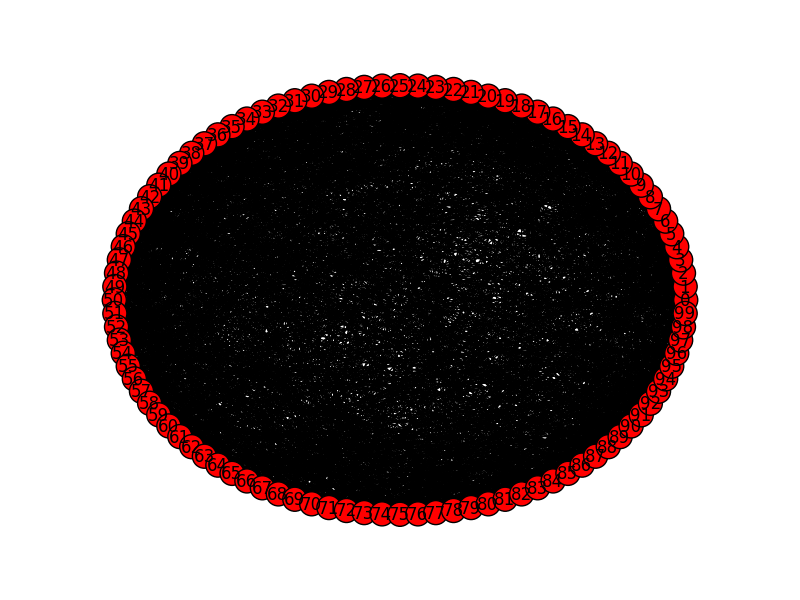
\includegraphics[scale=0.5]{./images/sim1_completedMessage_complete.png}
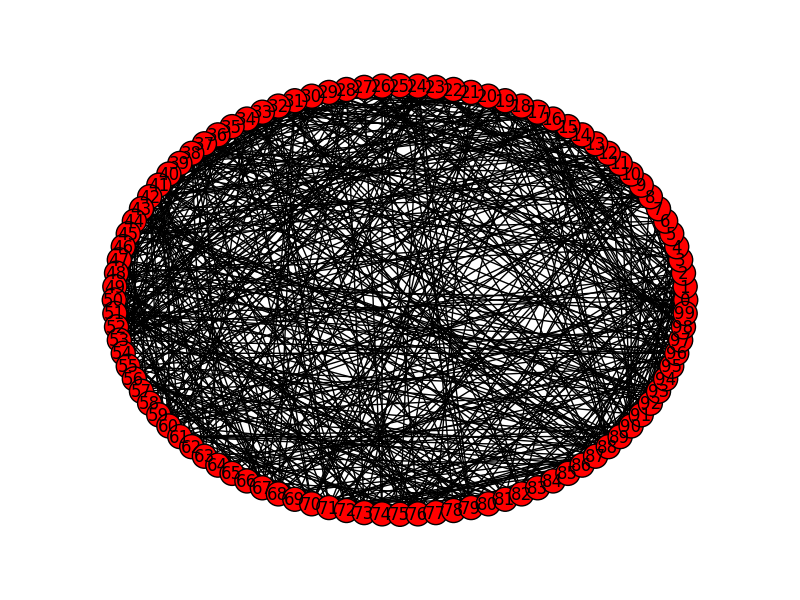
\includegraphics[scale=0.5]{./images/sim1_completedMessage_tx.png}
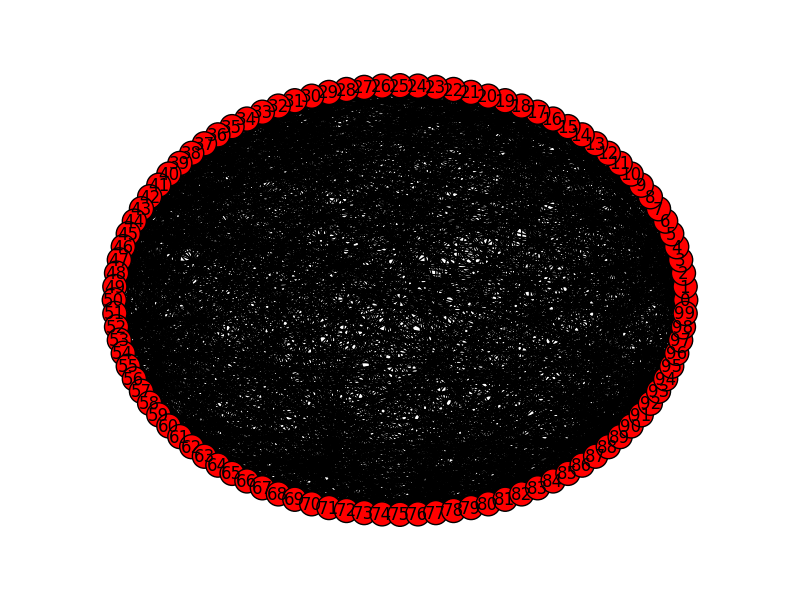
\includegraphics[scale=0.5]{./images/sim1_completedMessage_chaff.png}
\caption{The top figure shows the flow of both dummy messages and forwarded transactions from Experiment \#1, the middle figure shows only the transaction messages, and the bottom figure shows the cover traffic. Nodes have directed edges between them if some message was sent between them during the lifetime of the simulation. The coverage of nodes is clearly uniformly distributed, as desired.}
\label{fig:flow}
\end{center}
\end{figure*}


% cover traffic generation rate (random variable)
% mix buffer delay (random variable)
% circuit length (fixed)
% mix buffer size (fixed)
% encoded transaction size


\section{Related Cryptocurrencies} \label{sec:related}
Although Bitcoin is inarguably the most popular cryptocurrency to date, it is by no means the first such technology proposed. Other popular variants include DigiCash \cite{digicash}, E-Cash \cite{ecash}, HashCash \cite{hashcash}, Namecoin \cite{namecoin}, Peercoin \cite{peercoin}, Litecoin \cite{litecoin}, and Ripple \cite{ripple}. In this section we briefly describe some of these variants with respect to their anonymity properties. Our discussion begins with E-Cash \cite{ecash}.

Chaum, Fiat, and Naor’s offered two methods to create untraceable electronic cash. Both methods require a central bank organization. In all methods, the coins that are issued by the bank are blinded in a way to prevent the bank from identifying the source of honestly spent coins. The first method uses “untraceable coins” in that each transaction is of set amounts. Alice creates random commitments and sends them to the bank. The bank uses a subset of those commitments to create cryptographic coins by signing them. The bank then sends those coins to Alice after decrementing the amount from Alice’s account.  Everyone can verify the coin’s structure and the bank’s signature. Alice can then spend those coins to pay Bob. To do so, Alice sends Bob the information on the coin as well as a zero-knowledge proof that Alice initiated the creation of the coin. When Bob tries to redeem the coin with the bank, Bob sends both pieces of information to the bank. The bank will not have enough information to identify the coin came from Alice unless Alice tries to double spend. In that case, there is a high probability one of the challenges in the zero-knowledge proofs from the merchants will be different allowing the bank to reconstruct Alice’s identity. This method underpins the DigiCash system.

\begin{figure}
\begin{center}
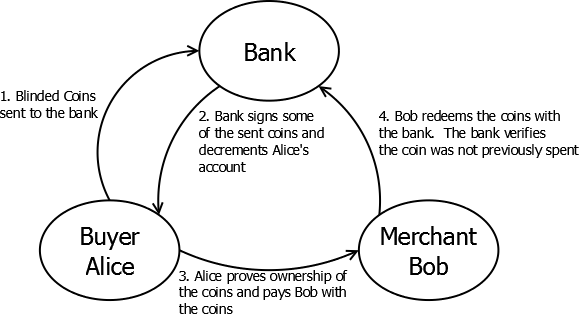
\includegraphics[scale=0.30]{images/digicash.png}
\caption{Digicash protocol.}
\label{fig:tor-end-to-end}
\end{center}
\end{figure}

The second method outlined is ``untraceable checks''.  The idea builds upon the “untraceable coins” idea by giving Alice has a roll of coins.  Alice can spend them by indexing the roll of coins by the purchase amount and revealing that to the merchant.  Alice is then refunded the rest of the amount by the bank by creating a separate transaction to pay herself.

Compact E-Cash builds upon the framework that Chaum creates with Untraceable Electronic Cash by creating a coin that can be used repeatedly a limited number of times. The system is comprised of a “withdrawal protocol”, a “spending protocol”, and a “double spending” check.  The withdrawal protocol involves the user creating a private key as well as the coin’s serial number and blinding value. The bank then signs the values and decrements the user’s account accordingly. The spending protocol has the user give the merchant the coin’s serial number, the merchant’s random number challenge, and a double-spending value based on the user’s private key, the random number challenge, and the blinding value.  The user also gives the merchant two non-interactive proofs.  The first proof is that the committed coin was signed by the bank.  The second proof verifies that the coin’s serial number and double spending number correspond to the commitment as well. The merchant then reveals this information to the bank for payment. In order to protect the user’s privacy, the serial number that is revealed to the merchant is encrypted using the user’s private key. In order to prevent the user from cheating, if the same coin is used over the limited number of uses, the bank is able to infer the secret key of the user, decrypt the serial number of the coin, and identify the user. This also means that the user can re-use coins a number of times without the bank being able to identify the user.
 
The Compact E-Cash system allows for users to create coins that can be used multiple times. The coins do not reveal the spending habits of the user if the user does not try to cheat and re-use the same coin too many times. The drawbacks are that there must be a central bank to issue coins and verify transactions. Also, each time a coin is used is a separate transaction even if the user spends multiple coins with the same merchant.

In both systems, privacy is maintained by blinded coins. If the user uses the system honestly and does not double spend, then the bank cannot reveal the identity of the user based on the coins used. Furthermore, because the coins are indistinguishable, the bank is unable to create profiles based on the location the coins were spent.

A mature form of the “untraceable coins” is the Mondex Smart Card. The bank issues secure cards embedded with an integrated circuit. The cards store “value” on the card. The “value” is incremented when money is transferred onto the card and decremented when the card is used for payment or deposit. In essence, if Alice pays Bob 5 coins, Alice’s card will destroy 5 coins and Bob’s card will create 5 coins. This makes the individual coins impossible to track. However, both Alice and Bob’s cards will have a transaction ledger that ties Alice’s and Bob’s cards to the transaction. Similar to a Bitcoin address, the card provides limited privacy as it separates the user from the coins being spent. However, merchants are able to create purchasing profiles based on transaction logs and the card’s internal identification. Furthermore, the system does not prevent merchants from sharing purchasing information with the issuing bank to match card identification numbers with an identity. In this way, the Mondex Smart Card system is less anonymous than other cryptocurrencies and does not provide any guarantees of privacy.

HashCash was originally designed to stop the waste or abuse of internet resources. HashCash requires the actor, Alice, to provide a proof-of-work before allowing an action such as sending an email. The idea is to add a cost to the action to prevent abuse. HashCash now has been incorporated into Bitcoin and similar cryptocurrency systems in the mining process as the proof-of-work protocol, but is not used as a currency system by itself. There are three protocols and two public variables in the original interactive HashCash system. The public variables are a hash function, $H(\cdot)$, and the length parameter $w$. In the Challenge protocol, the server, Bob, sends Alice the service name $s$ and a random challenge value $c$. Alice runs the Mint protocol to run a brute-force search for the value $x$. The hash of $s|c|x$, where $|$ represents concatenation, creates a value with $w$ leading zeroes. After Alice sends $x$ to Bob, Bob runs the Verify protocol to verify Alice’s work. If Verify succeeds, Alice is allowed to perform her action using the requested service. HashCash improvements include replacing the service name and challenge with a fixed output string and requiring Alice to find a collision. The proof-of-work can be considered a currency as it is used to create a transaction. If used in this way, HashCash does provide slightly better privacy than Bitcoins. Proofs-of-work are public knowledge, but HashCash does not have a ledger and therefore new nodes do not have access to the history of work.

\begin{figure}
\begin{center}
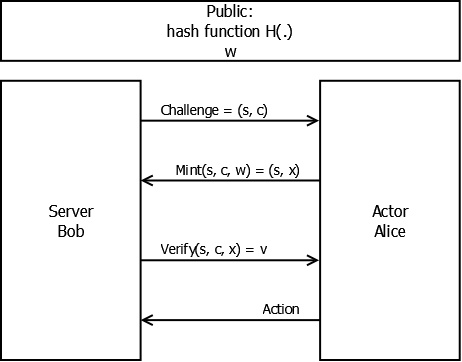
\includegraphics[scale=0.40]{images/hashcash.png}
\caption{Hashcash protocol.}
\label{fig:tor-end-to-end}
\end{center}
\end{figure}

Other alternative cryptocurrencies are based off the Bitcoin system, but only Zerocoin increases privacy. The other systems do not improve or reduce the privacy as compared to Bitcoin. Litecoin is the most similar to Bitcoin as it only differs in a few aspects. The first difference is that Litecoin uses scrypt instead of SHA-256, which is used in Bitcoin. Second, Litecoin has faster block times which decreases the time needed for a transaction confirmation. Finally, Litecoin increases the total number of coins available to be mined. Peercoin combines the HashCash proof-of-work method of mining coins with a second method, proof-of-stake. Proof-of-stake uses the notion of coin age. The coin age of a wallet is the sum of the lengths of time since a coin’s previous transaction. If Alice received 4 coins 2 days ago, then her wallet’s coin age would be 8 coin-days. In proof-of-stake, one hash per unspent wallet-output is created each second. Whereas the proof-of-work protocol uses a fixed hash target, proof-of-stake uses a variable hash target that scales inversely with coin age. If Alice finds an accepted value, she creates a transaction paying herself and is awarded one percent of her transaction as a reward. Being that her coins were used in a transaction, the mining process resets the coin age of Alice’s wallet. Namecoin is a cryptocurrency based off Bitcoin in the sense that the coins are used to register and transfer domain names. Namecoin is designed as a decentralized DNS. The ledger, which already contains coin transactions, will also contain DNS transactions such as the creation or purchase of a domain name and the associated IP address.

Unlike the previous cryptocurrencies which are based on the transference of “value”, Ripple is based on the transference of “debt”. Ripple is comprised of two parts. The first part involves a web-of-trust between nodes. Alice determines how much she trusts Bob and Charlie and then extends the maximum debt she is willing to accept from them. Suppose Charlie owes Alice 5 coins and Alice wanted to pay Bob 5 coins, but Bob only trusts Alice with a debt of 2 coins. If Bob trusts Charlie with a debt of 3 coins, Alice can send an IOU for 2 coins from her and an IOU for 3 coins from Charlie. Bob receives an IOU totaling 5 coins from which he can collect from Alice and Charlie at a later date or use to make payments to someone else.

\begin{figure*}[ht]
\begin{center}
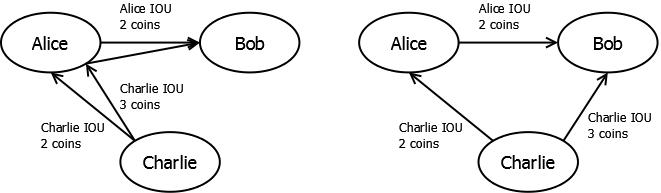
\includegraphics[scale=0.40]{images/ripple.png}
\caption{Ripple debt network.}
\label{fig:tor-end-to-end}
\end{center}
\end{figure*}

The second part of Ripple is to facilitate transactions where no web-of-trust exists. This is done through “gateway” nodes. Gateways act as publically known trusted nodes analogous to banks. If Alice wanted to pay Bob 5 coins, but Bob only trusts a gateway, then Alice can send 5 coins to the gateway and the gateway will credit Bob 5 coins. Unlike the first part of Ripple, gateways use stores of “value” instead of debt. Ripple is as private as Bitcoins as transfers of debt or credit between addresses is public knowledge, but no registry ties addresses to people. The exception is if Ripple deals with real world currency. Ripple is currency agnostic and therefore gateways are free to use real world currency as an exchange medium. In this case, gateways require personal information from the user and are able to link users to addresses and transactions.



\begin{thebibliography}{1}

\bibitem{bitcoin} Satoshi Nakamoto. Bitcoin: A Peer-to-Peer Electronic Cash System. \emph{Consulted} 1 (2008).

\bibitem{Chaum81-Mix} David L. Chaum. Untraceable electronic mail, return addresses, and digital pseudonyms. \emph{Communications of the ACM} 24(2) (1981), 84-90.

\bibitem{tarzan} Michael J. Freedman and Robert Morris. Tarzan: A Peer-to-Peer Anonymizing Network Layer. In \emph{Proceedings of the 9th ACM conference on Computer and Communications Security}, ACM (2002).

\bibitem{AnonymityTerms} A. Pfitzmann AND M. K\o{o}hntopp. Anonymity, Unobservability and Pseudonymity — A Proposal for Terminology. \emph{In Federrath} 12, 1-9.

\bibitem{kaminsky} Dan Kaminsky. Black Ops of TCP/IP Presentation. \emph{Black Hat, Chaos Communication Camp} (2011).

\bibitem{chaumain} David L. Chaum. Blind Signatures for Untraceable Payments. \emph{Crypto} 82 (1982).

\bibitem{zerocoin} Ian Miers, Christina Garman, Matthew Green, Aviel D. Rubin. Zerocoin: Anonymous Distributed E-Cash from Bitcoin. \emph{IEEE Symposium on Security and Privacy} (2013).

\bibitem{bitcoin-tor-wiki} Tor. Bitcoin Wiki. Available online at \url{https://en.bitcoin.it/wiki/Tor}. Last accessed: 1/25/14.

\bibitem{nist-prng} Elaine Barker and John Kelsey. Recommendation for Random Number Generation Using Deterministic Random Bit Generators. 2012. Available online at: \url{http://csrc.nist.gov/publications/nistpubs/800-90A/SP800-90A.pdf}. Last accessed: 2/10/14. 

\bibitem{tor} Roger Dingledine, Nick Mathewson, and Paul Syverson. Tor: The Second-Generation Onion Router. \emph{Naval Research Lab Washington DC} (2004).

\bibitem{jyaml} JYaml - Yaml library for the Java language. Available online at \url{http://jyaml.sourceforge.net/}. Last accessed: 2/10/14. 

% \bibitem{Androulaki12-privacy} Elli Androulaki, Ghassan O. Karame, Marc Roeschlin, Tobias Scherer, and Srdjan Capkun. Evaluating User Privacy in Bitcoin. \emph{IACR Cryptology ePrint Archive} 596 (2012).

% \bibitem{Shamir13-bitcoingraph} Dorit Ron and Adi Shamir. Quantitative Analysis of the Full Bitcoin Transaction Graph. \emph{IACR Cryptology ePrint Archive} 584 (2012).

% \bibitem{ReidHarrigan13} Fergal Reid and Martin Harrigan. An Analysis of Anonymity in the Bitcoin System. \emph{Security and Privacy in Social Networks}, Springer New York (2013), 197-223.

\bibitem{BetterToBitter} Simon Barber, Xavier Boyen, Elaine Shi, and Ersin Uzun. Bitter to Better -- How to Make Bitcoin a Better Currency. \emph{Financial Cryptography and Data Security}, Springer Berlin Heidelberg (2012), 399-414.

% \bibitem{Fistful12} Sarah Meiklejohn, Marjori Pomarole, Grant Jordan, Kirill Levchenko, Damon McCoyy, Geoffrey M. Voelker, and  Stefan Savage. A Fistful of Bitcoins: Characterizing Payments Among Men with No Names. In \emph{Proceedings of the 2013 Conference on Internet Measurement Conference}, ACM (2013).

% \bibitem{coinjoin} G. Maxwell. Coinjoin: Bitcoin Privacy for the Real World. Available online at \url{https://bitcointalk.
% org/index.php?topic=279249.0}. Last accessed: 1/31/14.

\bibitem{pinocchio} George Danezis, C\'{e}dric Fournet, Markulf Kohlweiss, Bryan Parno. Pinocchio Coin: Building Zerocoin from a Succinct Pairing-Based Proof System. In \emph{Proceedings of the First ACM Workshop on Language Support for Privacy-Enhancing Technologies}, ACM (2013).

\bibitem{mixcoin} Joseph Bonneau, Arvind Narayan, Andrew Miller, Jeremy Clark, and Joshua A. Kroll. Mixcoin - Anonymity for Bitcoin with accountable mixes. Preprint available online at: \url{http://cs.umd.edu/~amiller/mix.pdf}.

\bibitem{nist-curves} Darrel Hankerson and Alfred Menezes. NIST Elliptic Curves. \emph{Encyclopedia of Cryptography and Security} (2011), 843-844.

% \bibitem{nist-beacon} NIST Randomness Beacon. Available online at: \url{http://www.nist.gov/itl/csd/ct/nist_beacon.cfm}. Last accessed: 2/5/14.

\end{thebibliography}

\appendix 
\addcontentsline{toc}{chapter}{APPENDICES}

\section{Extended Simulation Results}
Table \ref{tab:extended-results} contains an extended set of experimental results acquired from our simulator. Observe that in all cases the average message latency, measured in discrete time epochs, is quite reasonable since a single epoch is approximately equal to 0.1s. For example, a message latency of 9918.31 epochs is approximately equivalent to 992s, which is roughly 16 minutes. Since there are no real-time constraints on transaction broadcast introduction, and double-spending is prevented by miners who verify the first instance of a broadcasted transaction, we believe such a delay is reasonable.
\begin{table*}
\begin{center}
\caption{Extended simulation results including average message latency and traffic generation rates ($\pi$ and $\sigma$).}
\label{tab:extended-results}
    \begin{tabular}{|c|c|c|c|c|c|c|c|} \hline
    $n$ & $\pi$ & $\sigma$ & {\bf Avg. Latency} & {\bf Avg. Chaff Generated} & {\bf Avg. Transactions Encoded} & {\bf Avg. Forwarded Messages} & {\bf Avg. Retries} \\ \hline
  % N, pi, sigma, avgLatency, avgChaffComputations, avgTxComputtions, avgForwarded, avgRetries
2000 & 200 & 1000 & 9918.31 & 343.35 & 7.78 & 180.79 & 0.96 \\
2000 & 200 & 1000 & 2780.40 & 488.42 & 15.91 & 179.17 & 0.00 \\
2000 & 200 & 1000 & 3577.19 & 1082.87 & 31.84 & 415.03 & 0.00 \\
2000 & 200 & 1000 & 10218.64 & 4528.39 & 96.28 & 2758.08 & 0.75 \\
2000 & 200 & 1000 & 18528.48 & 16059.35 & 273.23 & 5814.22 & 1.88 \\
2000 & 200 & 1000 & 9121.64 & 324.26 & 7.97 & 159.93 & 0.99 \\
2000 & 2000 & 5000 & 3296.00 & 148.19 & 42.54 & 29.80 & 0.00 \\
2000 & 2000 & 5000 & 46249.89 & 6916.45 & 1053.30 & 3483.64 & 6.34 \\
2000 & 2000 & 5000 & 3972.31 & 198.35 & 47.36 & 66.26 & 0.00 \\
2000 & 2000 & 5000 & 32704.14 & 3603.02 & 568.94 & 2599.06 & 5.01 \\
2000 & 2000 & 5000 & 3970.25 & 197.43 & 47.36 & 66.19 & 0.00 \\
2000 & 2000 & 5000 & 33929.58 & 3890.12 & 605.98 & 2673.71 & 5.40 \\
2000 & 2000 & 5000 & 56236.27 & 11361.13 & 1692.57 & 6402.18 & 10.93 \\
2000 & 2000 & 5000 & 3830.50 & 178.52 & 47.38 & 52.89 & 0.00 \\
200 & 200 & 1000 & 15411.71 & 3592.23 & 66.20 & 3030.34 & 15.49 \\
200 & 200 & 1000 & 35780.14 & 6052.75 & 97.88 & 3784.15 & 11.45 \\
200 & 200 & 1000 & 49408.82 & 5255.79 & 80.54 & 2464.30 & 5.83 \\
200 & 200 & 1000 & 15041.98 & 4424.46 & 87.00 & 3797.90 & 4.09 \\
200 & 200 & 1000 & 34192.21 & 11456.77 & 198.34 & 6859.86 & 5.28 \\
200 & 200 & 1000 & 44278.54 & 18685.20 & 285.63 & 7797.51 & 5.05 \\
200 & 200 & 1000 & 10695.88 & 3319.69 & 67.26 & 2208.28 & 0.79 \\
200 & 200 & 1000 & 31071.47 & 19921.87 & 348.41 & 11336.27 & 4.51 \\
200 & 200 & 1000 & 15859.56 & 29871.07 & 567.61 & 25852.14 & 8.74 \\
200 & 200 & 1000 & 35890.42 & 101208.49 & 1591.11 & 60676.89 & 15.83 \\
200 & 2000 & 5000 & 22007.83 & 95.52 & 17.23 & 79.04 & 4.07 \\
200 & 2000 & 5000 & 46316.93 & 218.59 & 33.93 & 123.64 & 4.01 \\
200 & 2000 & 5000 & 70855.82 & 337.74 & 50.17 & 156.51 & 3.87 \\
200 & 2000 & 5000 & 16385.33 & 371.22 & 67.33 & 347.38 & 3.58 \\
200 & 2000 & 5000 & 35475.20 & 814.33 & 128.44 & 570.80 & 3.66 \\
200 & 2000 & 5000 & 58155.07 & 1363.12 & 201.09 & 647.35 & 3.91 \\
200 & 2000 & 5000 & 16249.05 & 760.73 & 135.37 & 643.99 & 3.63 \\
200 & 2000 & 5000 & 36339.58 & 1841.39 & 286.72 & 1150.79 & 4.28 \\
200 & 2000 & 5000 & 59842.71 & 2883.20 & 427.02 & 1265.85 & 4.24 \\
200 & 2000 & 5000 & 15539.04 & 1162.00 & 202.93 & 1004.22 & 3.33 \\
200 & 2000 & 5000 & 36597.48 & 2641.06 & 411.73 & 1548.01 & 4.09 \\
200 & 2000 & 5000 & 56703.05 & 4307.92 & 635.29 & 1905.60 & 4.21 \\
200 & 2000 & 5000 & 32079.91 & 37.29 & 6.80 & 16.56 & 1.50 \\
200 & 2000 & 5000 & 43757.67 & 81.37 & 12.95 & 16.95 & 1.42 \\
200 & 2000 & 5000 & 16949.92 & 152.76 & 27.91 & 89.56 & 1.51 \\
200 & 2000 & 5000 & 34974.36 & 448.44 & 71.17 & 135.03 & 1.91 \\
200 & 2000 & 5000 & 62589.00 & 792.99 & 120.90 & 163.91 & 2.15 \\
200 & 2000 & 5000 & 15324.64 & 392.49 & 71.88 & 251.08 & 1.78 \\
200 & 2000 & 5000 & 34836.53 & 834.26 & 133.21 & 268.63 & 1.79 \\
200 & 2000 & 5000 & 56656.67 & 1268.65 & 193.09 & 259.45 & 1.73 \\
200 & 2000 & 5000 & 15666.90 & 510.83 & 93.52 & 318.95 & 1.55 \\
200 & 2000 & 5000 & 31933.98 & 957.48 & 151.80 & 271.72 & 1.39 \\
200 & 2000 & 5000 & 53678.33 & 1613.27 & 243.98 & 324.57 & 1.49 \\ \hline
    \end{tabular}
  \end{center}
\end{table*}


% that's all folks
\end{document}


